% ────────────────────────────────────────────
%  Masterarbeit — Hauptdokument
%  Kompilieren: Strg+S oder Strg+Enter  ·  Literatur: Bibliothek-Tab
% ────────────────────────────────────────────
\documentclass[
  11pt, a4paper, twoside, openright,
  parskip=half, headings=standardclasses, numbers=noenddot,
  bibliography=totoc, listof=totoc
]{scrreprt}

% ── Sprache ─────────────────────────────────
% Für korrekte deutsche Silbentrennung: Paket texlive-langgerman installieren.
\IfFileExists{ngerman.ldf}{\usepackage[ngerman]{babel}}{%
  \usepackage[english]{babel}%
  \AtBeginDocument{% Deutsche Bezeichnungen, falls babel-german (texlive-langgerman) fehlt.
\renewcommand{\contentsname}{Inhaltsverzeichnis}
\renewcommand{\listfigurename}{Abbildungsverzeichnis}
\renewcommand{\listtablename}{Tabellenverzeichnis}
\renewcommand{\bibname}{Literaturverzeichnis}
\renewcommand{\figurename}{Abbildung}
\renewcommand{\tablename}{Tabelle}
\renewcommand{\chaptername}{Kapitel}
\renewcommand{\appendixname}{Anhang}
\renewcommand{\abstractname}{Kurzfassung}
\renewcommand{\today}{\number\day.~\ifcase\month\or Jänner\or Februar\or März\or April\or Mai\or Juni\or Juli\or August\or September\or Oktober\or November\or Dezember\fi~\number\year}
}}
\usepackage[T1]{fontenc}
\usepackage[utf8]{inputenc}
\usepackage{csquotes}

% ── Schrift & Satz ──────────────────────────
\usepackage{libertinus-type1}
\usepackage[scale=0.92]{sourcesanspro}
\usepackage{microtype}
\usepackage[top=28mm, bottom=30mm, inner=30mm, outer=26mm]{geometry}
\usepackage{setspace}\onehalfspacing
\addtokomafont{disposition}{\sffamily}
\addtokomafont{chapter}{\color{akzent}}

% ── Mathematik, Grafik, Tabellen ────────────
\usepackage{amsmath, amssymb, mathtools}
\usepackage{graphicx}\graphicspath{{abbildungen/}}
\usepackage{booktabs, tabularx}
\usepackage[font=small, labelfont={bf,sf}]{caption}
\usepackage{subcaption}
\usepackage[locale=DE]{siunitx}
\usepackage{xcolor}
\definecolor{akzent}{HTML}{1F4E79}
\usepackage{tikz}
\usepackage{pgfplots}\pgfplotsset{compat=1.18}
\usepackage[shortlabels]{enumitem}

% ── Literatur (natbib + BibTeX) ─────────────
\usepackage[round, authoryear]{natbib}
\bibliographystyle{plainnat}

% ── Links & Querverweise ────────────────────
\usepackage[hidelinks, pdfusetitle]{hyperref}
\usepackage[nameinlink, noabbrev, ngerman]{cleveref}

% ── Metadaten ───────────────────────────────
\newcommand{\arbeitstitel}{Hopfen, Hefe, Hochgenuss}
\newcommand{\untertitel}{Der Einfluss der Gärtemperatur auf das Aromaprofil obergäriger Biere}
\newcommand{\autorin}{Norbert Winter}
\newcommand{\betreuung}{Univ.-Prof. Dr. Hilde Malzbauer (fiktiv)}
\newcommand{\institut}{Institut für Brau- und Gärungstechnologie (fiktiv)}
\newcommand{\universitaet}{Technische Universität Graz}
\newcommand{\studium}{Masterstudium Lebensmitteltechnologie}

\title{\arbeitstitel}
\author{\autorin}

\begin{document}

\begin{titlepage}
  \sffamily
  \begin{tikzpicture}[remember picture, overlay]
    \fill[akzent] (current page.north west) rectangle ([yshift=-9mm]current page.north east);
  \end{tikzpicture}
  \vspace*{22mm}

  {\large\color{akzent}\textbf{MASTERARBEIT}}\par
  \vspace{10mm}
  {\fontsize{26}{32}\selectfont\bfseries \arbeitstitel\par}
  \vspace{5mm}
  {\Large\color{black!65} \untertitel\par}

  \vfill
  {\Large \autorin}\par
  \vspace{2mm}
  zur Erlangung des akademischen Grades\\
  \textbf{Diplom-Ingenieur} im \studium

  \vspace{14mm}
  \begin{tabular}{@{}ll}
    \textbf{Betreuung:} & \betreuung \\
    \textbf{Institut:}  & \institut \\
  \end{tabular}

  \vspace{14mm}
  {\color{akzent}\rule{\linewidth}{0.8pt}}\par
  \universitaet \hfill Graz, \today
\end{titlepage}
\cleardoublepage


\pagenumbering{roman}
\chapter*{Kurzfassung}
\addcontentsline{toc}{chapter}{Kurzfassung}

Obergärige Biere verdanken ihr fruchtiges Aroma vor allem den Estern und höheren
Alkoholen, die Hefen während der Gärung bilden. Diese (erfundene) Arbeit untersucht,
wie stark die Gärtemperatur dieses Aromaprofil prägt. In zwölf Versuchssuden eines
Pale Ale wurde die Temperatur zwischen \SI{16}{\celsius} und \SI{24}{\celsius}
variiert. Die Ergebnisse zeigen einen nahezu linearen Anstieg des Isoamylacetats
-- dem typischen Bananenaroma -- um rund \SI{38}{\percent} je \SI{4}{\kelvin}.
Eine Verkostung mit 24 Personen bestätigt: wärmer vergorene Biere werden als
fruchtiger, aber auch als weniger \enquote{sauber} wahrgenommen.

\chapter*{Abstract}
\addcontentsline{toc}{chapter}{Abstract}

This (fictional) thesis investigates how fermentation temperature shapes the aroma
profile of top-fermented beers. Isoamyl acetate increased by roughly 38\,\% per 4\,K.

\tableofcontents
\cleardoublepage
\pagenumbering{arabic}

\chapter{Einleitung}
\label{ch:einleitung}

\section{Motivation}
Bier ist eines der ältesten Lebensmittel der Menschheit. Spätestens seit dem
Reinheitsgebot von 1516 besteht es in Mitteleuropa aus nur vier Zutaten: Wasser,
Malz, Hopfen und Hefe \citep{hopfner2019reinheit}. Trotz dieser Einfachheit
unterscheiden sich Biere enorm in Geschmack und Geruch -- und ein großer Teil
dieser Vielfalt entsteht nicht im Sudhaus, sondern im Gärtank \citep{malz2021ester}.

Craft-Brauereien experimentieren daher zunehmend mit Gärparametern. Gleichzeitig
fehlt es an \textbf{systematischen Daten}, wie stark einzelne Parameter das
Aroma tatsächlich verändern.

\section{Forschungsfragen}
\begin{enumerate}[label=\textbf{F\arabic*}]
  \item Wie verändert sich die Konzentration aromaaktiver Ester mit der Gärtemperatur?
  \item Ab welcher Temperatur nehmen Verkosterinnen und Verkoster den Unterschied wahr?
  \item Lässt sich das Aromaprofil mit einem einfachen Modell vorhersagen?
\end{enumerate}

\section{Aufbau der Arbeit}
\Cref{ch:grundlagen} erklärt die Biochemie der Gärung, \cref{ch:methodik}
beschreibt die Versuchssude, \cref{ch:ergebnisse} präsentiert Messwerte und
Verkostung, und \cref{ch:fazit} gibt einen Ausblick -- inklusive Rezeptempfehlung.

\chapter{Grundlagen}
\label{ch:grundlagen}

\section{Was Hefe eigentlich macht}
Während der Gärung wandelt die Hefe \emph{Saccharomyces cerevisiae} vergärbaren
Zucker in Ethanol und Kohlendioxid um:
\begin{equation}
  \mathrm{C_6H_{12}O_6} \;\longrightarrow\; 2\,\mathrm{C_2H_5OH} + 2\,\mathrm{CO_2}
  \label{eq:gaerung}
\end{equation}
Nebenbei entstehen hunderte Aromastoffe. Besonders wichtig sind:
\begin{itemize}
  \item \textbf{Ester} wie Isoamylacetat (Banane) und Ethylhexanoat (Apfel),
  \item \textbf{höhere Alkohole} wie Isoamylalkohol (lösungsmittelartig),
  \item \textbf{Phenole} wie 4-Vinylguajakol (Gewürznelke, typisch für Weizenbier).
\end{itemize}

\section{Temperatur als Stellschraube}
Die Esterbildung folgt näherungsweise einer Arrhenius-Beziehung
\citep{gerstner2020kinetik}:
\begin{equation}
  k(T) = A \cdot \exp\!\left(-\frac{E_a}{R\,T}\right)
  \label{eq:arrhenius}
\end{equation}
Nach \cref{eq:arrhenius} sollte eine höhere Temperatur die Bildung deutlich
beschleunigen -- wie stark, ist für obergärige Hefen jedoch kaum dokumentiert
\citep{malz2021ester, hefeling2018obergaerig}.

\chapter{Methodik}
\label{ch:methodik}

\section{Versuchssude}
Gebraut wurden zwölf identische Sude eines Pale Ale (Stammwürze \SI{12.5}{\degree P}),
aufgeteilt auf vier Temperaturstufen mit je drei Wiederholungen.

\begin{table}[htbp]
  \centering
  \caption{Rezeptur und Gärparameter (pro \SI{20}{\liter} Sud)}
  \label{tab:rezept}
  \begin{tabular}{lrl}
    \toprule
    Zutat / Parameter & Menge   & Einheit \\
    \midrule
    Pale-Ale-Malz     & 4{,}2   & kg \\
    Cascade-Hopfen    & 60      & g \\
    Obergärige Hefe   & 11{,}5  & g \\
    Gärtemperatur     & 16 -- 24 & \si{\celsius} \\
    Gärdauer          & 7       & Tage \\
    \bottomrule
  \end{tabular}
\end{table}

\section{Analytik und Verkostung}
Die Ester wurden per Gaschromatografie bestimmt. Zusätzlich bewerteten 24 Personen
die Biere blind nach Fruchtigkeit, Sauberkeit und Gesamteindruck
(Skala 1--9), siehe \cref{tab:rezept} für die Rahmenbedingungen.

\chapter{Ergebnisse}
\label{ch:ergebnisse}

\section{Esterbildung}
\Cref{fig:ester} zeigt den deutlichen Anstieg von Isoamylacetat mit der Temperatur.

\begin{figure}[htbp]
  \centering
  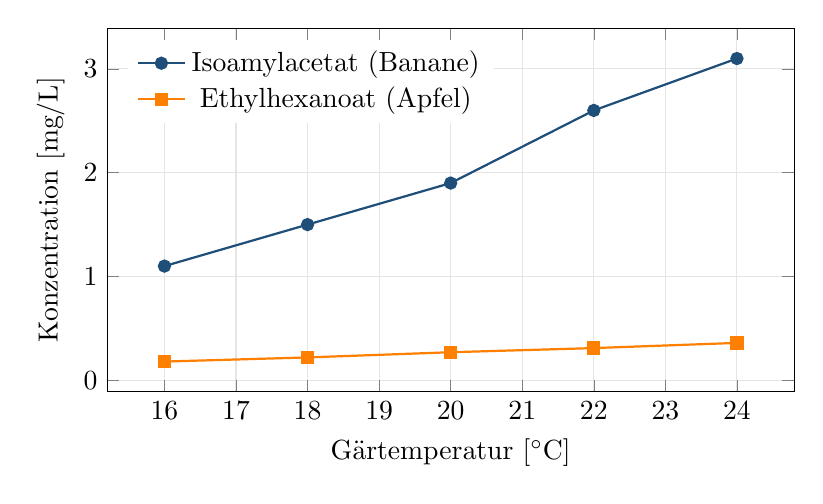
\begin{tikzpicture}
    \begin{axis}[
      width=0.85\linewidth, height=6.2cm,
      xlabel={Gärtemperatur [\si{\celsius}]}, ylabel={Konzentration [mg/L]},
      grid=major, grid style={black!10},
      legend pos=north west, legend style={draw=none},
      every axis plot/.append style={thick}
    ]
      \addplot[color=akzent, mark=*] coordinates {(16,1.1) (18,1.5) (20,1.9) (22,2.6) (24,3.1)};
      \addplot[color=orange, mark=square*] coordinates {(16,0.18) (18,0.22) (20,0.27) (22,0.31) (24,0.36)};
      \legend{Isoamylacetat (Banane), Ethylhexanoat (Apfel)}
    \end{axis}
  \end{tikzpicture}
  \caption{Esterkonzentration in Abhängigkeit der Gärtemperatur (Mittelwerte, $n=3$).}
  \label{fig:ester}
\end{figure}

\section{Verkostung}
Ab \SI{20}{\celsius} wurde der Unterschied von \SI{88}{\percent} der Personen
erkannt. Das bei \SI{18}{\celsius} vergorene Bier erhielt den besten
Gesamteindruck -- fruchtig, aber noch \enquote{sauber}.

\chapter{Fazit und Ausblick}
\label{ch:fazit}

\section{Zusammenfassung}
Die Gärtemperatur ist die wirkungsvollste und zugleich billigste Stellschraube für
das Aroma obergäriger Biere. Bereits \SI{4}{\kelvin} verändern das Esterprofil
stärker als eine Verdoppelung der Aromahopfengabe \citep{hopfner2019reinheit}.

\section{Ausblick}
\begin{itemize}
  \item Untersuchung weiterer Hefestämme, insbesondere Kveik-Hefen,
  \item Temperaturprofile statt konstanter Temperaturen,
  \item und natürlich: eine größere Verkostung.
\end{itemize}


\bibliography{references}

\appendix
\chapter{Messwerte}
\label{ch:anhang}
Alle Rohdaten dieser fiktiven Arbeit sind frei erfunden.


\end{document}
